\documentclass[border=8pt]{standalone}
\usepackage{pgfplots}
\pgfplotsset{compat=1.18}
\begin{document}
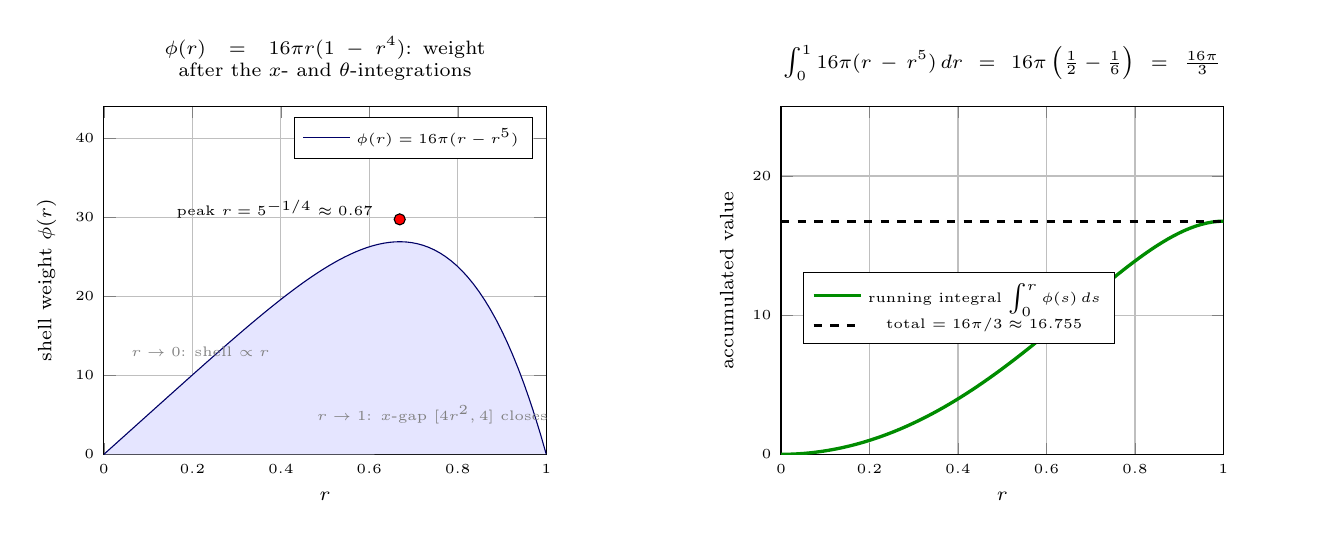
\begin{tikzpicture}
\begin{axis}[
    width=7.2cm, height=6.0cm, at={(0,0)},
    xlabel={$r$}, ylabel={shell weight $\phi(r)$},
    xmin=0, xmax=1, ymin=0, ymax=44,
    grid=major,
    title={$\phi(r)=16\pi r(1-r^{4})$: weight after the $x$- and $\theta$-integrations},
    legend style={font=\tiny, at={(0.97,0.97)}, anchor=north east},
    tick label style={font=\tiny}, label style={font=\scriptsize},
    title style={font=\scriptsize, align=center, text width=7cm}]
\addplot[blue!40!black, fill=blue!10, domain=0:1, samples=80] {16*pi*(x-x^5)};
\addlegendentry{$\phi(r)=16\pi(r-r^5)$}
\addplot[only marks, mark=*, mark options={fill=red}, forget plot] coordinates {(0.6687,29.72)};
\node[font=\tiny, anchor=east] at (axis cs:0.63,31.0) {peak $r=5^{-1/4}\approx0.67$};
\node[font=\tiny, gray, anchor=west, align=left] at (axis cs:0.04,13.0)
     {$r\to0$: shell $\propto r$};
\node[font=\tiny, gray, anchor=west, align=left] at (axis cs:0.46,5.0)
     {$r\to1$: $x$-gap $[4r^2,4]$ closes};
\end{axis}

\begin{axis}[
    width=7.2cm, height=6.0cm, at={(8.6cm,0)}, anchor=south west,
    xlabel={$r$}, ylabel={accumulated value},
    xmin=0, xmax=1, ymin=0, ymax=25,
    grid=major,
    title={$\int_0^1 16\pi(r-r^5)\,dr=16\pi\left(\frac{1}{2}-\frac{1}{6}\right)=\frac{16\pi}{3}$},
    legend style={font=\tiny, at={(0.05,0.42)}, anchor=west},
    tick label style={font=\tiny}, label style={font=\scriptsize},
    title style={font=\scriptsize, align=center, text width=7.2cm}]
\addplot[green!55!black, very thick, domain=0:1, samples=80] {16*pi*(x^2/2 - x^6/6)};
\addlegendentry{running integral $\int_0^r\phi(s)\,ds$}
\addplot[black, dashed, very thick, domain=0:1, samples=2] {16*pi/3};
\addlegendentry{total $=16\pi/3\approx16.755$}
\end{axis}
\end{tikzpicture}
\end{document}
